\section{Parallelism}

\subsection{Standard}

``Poor man parallelization'' is implemented. It can be used with the parameter: \verb+/MC/General/domains+ set to the number of threads. Default is 1.

This type of \idx{parallelization} is done by simple splitting of the $z$ axis, as can be seen in Fig.~\ref{fig:poor-parallelization} and running in a totally independent way such splits in different threads, with no communication at all between them during the annealing. Insertion and extraction of information is, nevertheless, transparent to the user, meaning that the user input (cascade, profile, anneal) and output (extract) commands will work as if there is only 1 domain.

This parallelization is optimal when a better statistics is needed and there is 1D or 2D symmetry in the system. Special care has to be taken to be be sure that each domain is big enough to represent the physics of the system simulated. For example, if a system requires at least 20\,nm in the z axis, a simulation with at least $20\times n$, being $n$ the number of threads, needs to be run, because each thread will run a simulation with $20\times n / n = 20$\,nm in the z axis.

Parallel execution is also possible using the new nonuniform mesh. The simulation area is divided along the Z axis, but only at the division planes. This division happens possibly in a uniform way. Should the linesz resolution be too coarse somewhere, a domain may end up with 0 Z-size. This happens for example when one sets 16 domains but has only 6 division planes along the Z axis.. In this case, MMonCa exits with an error message.

Note, however, nonuniform meshes don't support more than 1 subdomains.

Alternative ways of parallelization are being currently studied. If you want to have more information ask {\tt ignacio.martin@imdea.org}.

\begin{figure}
\begin{center}
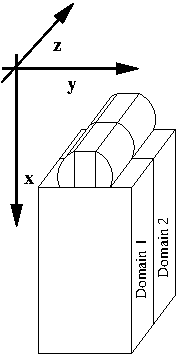
\includegraphics{images/poor-parallelization}
\end{center}
\caption{Simple parallelization splits the z domain in independent sub-domains and runs them isolated from each other. All input and output of information is transparent to the user.}
\label{fig:poor-parallelization}
\end{figure}

\subsection{Experimental}

Experimental parallelization based on the work of \cite{MARTINEZ-JCP08} has been implemented as explained in \cite{MARTIN-BRAGADO-NIMB15}. As explained in the cited paper, this parallelization works but should be used with extreme caution to avoid very slow simulations.
